\chapter{Introduction}
\label{sec:Introduction}

\paragraph{}

\indent In recent decades, understanding the state of sea ice has grown increasingly important. Sea ice analysis at large scales can provide valuable insight into the trajectory of climate change and at local scale has implications in fields like arctic navigation. Understanding sea-ice thickness in particular, is important for both of these applications.  For example, the thickness of the ice can be analyzed over time to track ice mass in relation to global warning or interpreted locally to predict shipping speed through ice-covered water \cite{sea-ice-properties}.

% Crop the image to better fit the page. Also include an image that contrasts this availability with the availability of any other remote sensed method.
\begin{wrapfigure}{R}{0.35\textwidth}
	\centering
	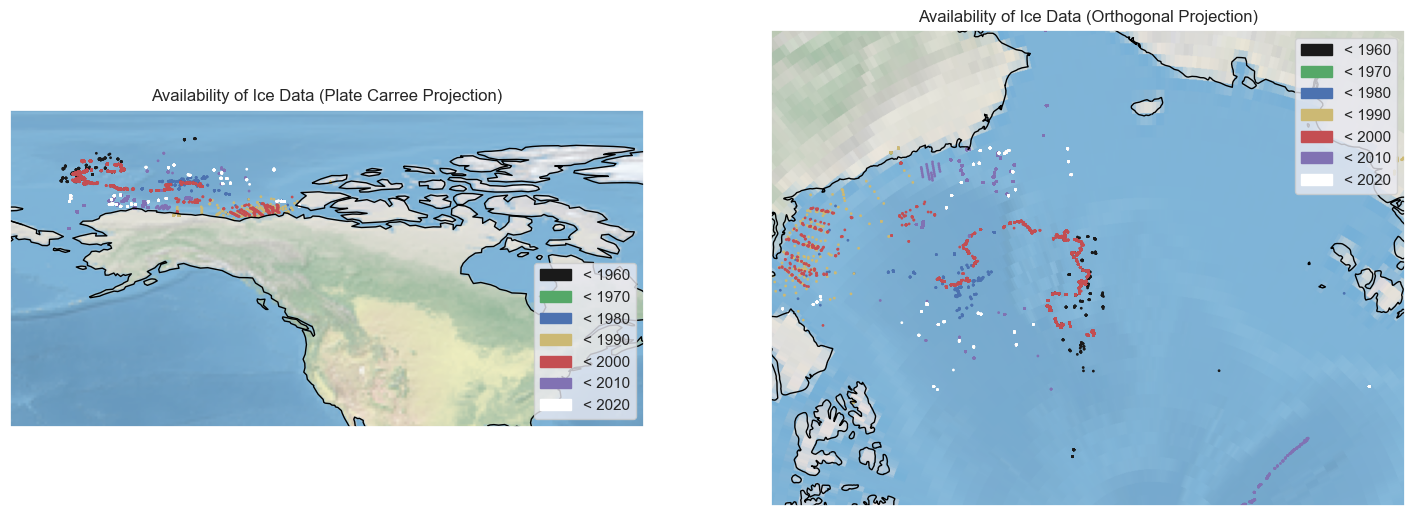
\includegraphics[width=0.5\textwidth]{../research-resources/in-situ/Plotted-Tracks.png}
	\caption{Historic In-Situ Data Availability in the Beaufort Sea Region}
	\label{fig:foobar}
\end{wrapfigure}


\indent Due to the harsh nature of the arctic, in-situ studies of arctic ice are infrequent both in time and space. Thus, most analyses depend heavily on remote sensing methods. These methods cumulatively provide magnitudes more data than in-situ measurements can achieve, but differ in modality, methodology and resolution. Synthetic Aperture Radar (SAR) and light detection and ranging (LiDAR) are some such modalities that survey the arctic region. Furthermore, organizations like the the National Aeronautics and Space Administration (NASA) and European Space Agency (ESA) freely provide this information through their constellation of satellites.


Each of these remote sensing methods have their individual strengths and limitations. ICESat-2 (IS-2), a NASA LiDAR satellite, features 6 separate lasers and works by emitting individual photons and timing their respective returns.
Praised for its precision, its readings are statistically corrected to adjust for ambient light, cloud occlusion (atmospheric scattering), snow and ice scattering, and the physical problem of first-photon bias \cite{ICESat-2-ATL10-Product}. It's lasers have a ground-surface footprint of 17 meters, demonstrating how local its sampling is. IS-2's statistical robustness offers valuable local observation with less than 5 meters of total geolocation error (mean \(+ 1\sigma\)) \cite{ICESat-2-Horizontal-Accuracy}.

In contrast to IS-2's highly accurate and local measurements, SAR imaging offers significantly more expansive data with a loss in local precision. SAR images Earth's surface by emitting radio waves and then reconstructing the surface composition based upon the return signal. The physical difference between photons and radio waves means that LiDAR's limitations with occlusion are actually imperceptible to SAR satellites. Radio waves permeate clouds and snow, and the reconstructed image is independent of light \cite{SAR-Info}. These weather independent properties make SAR an excellent modality to monitor sea ice especially during winter seasons, with satellites like Sentinel-2 (SN-2) from the ESA offering 290 kilometer swaths of imaging, at resolutions ranging between 10 and 60 meters \cite{Sentinel-2-Availability}. It's important to note that despite its extensiveness, SAR is more sensitive to physical factors like surface roughness, slant, and type, and also suffers from speckle noise \cite{SAR-Info}. 

\begin{figure}[h]
	\centering
	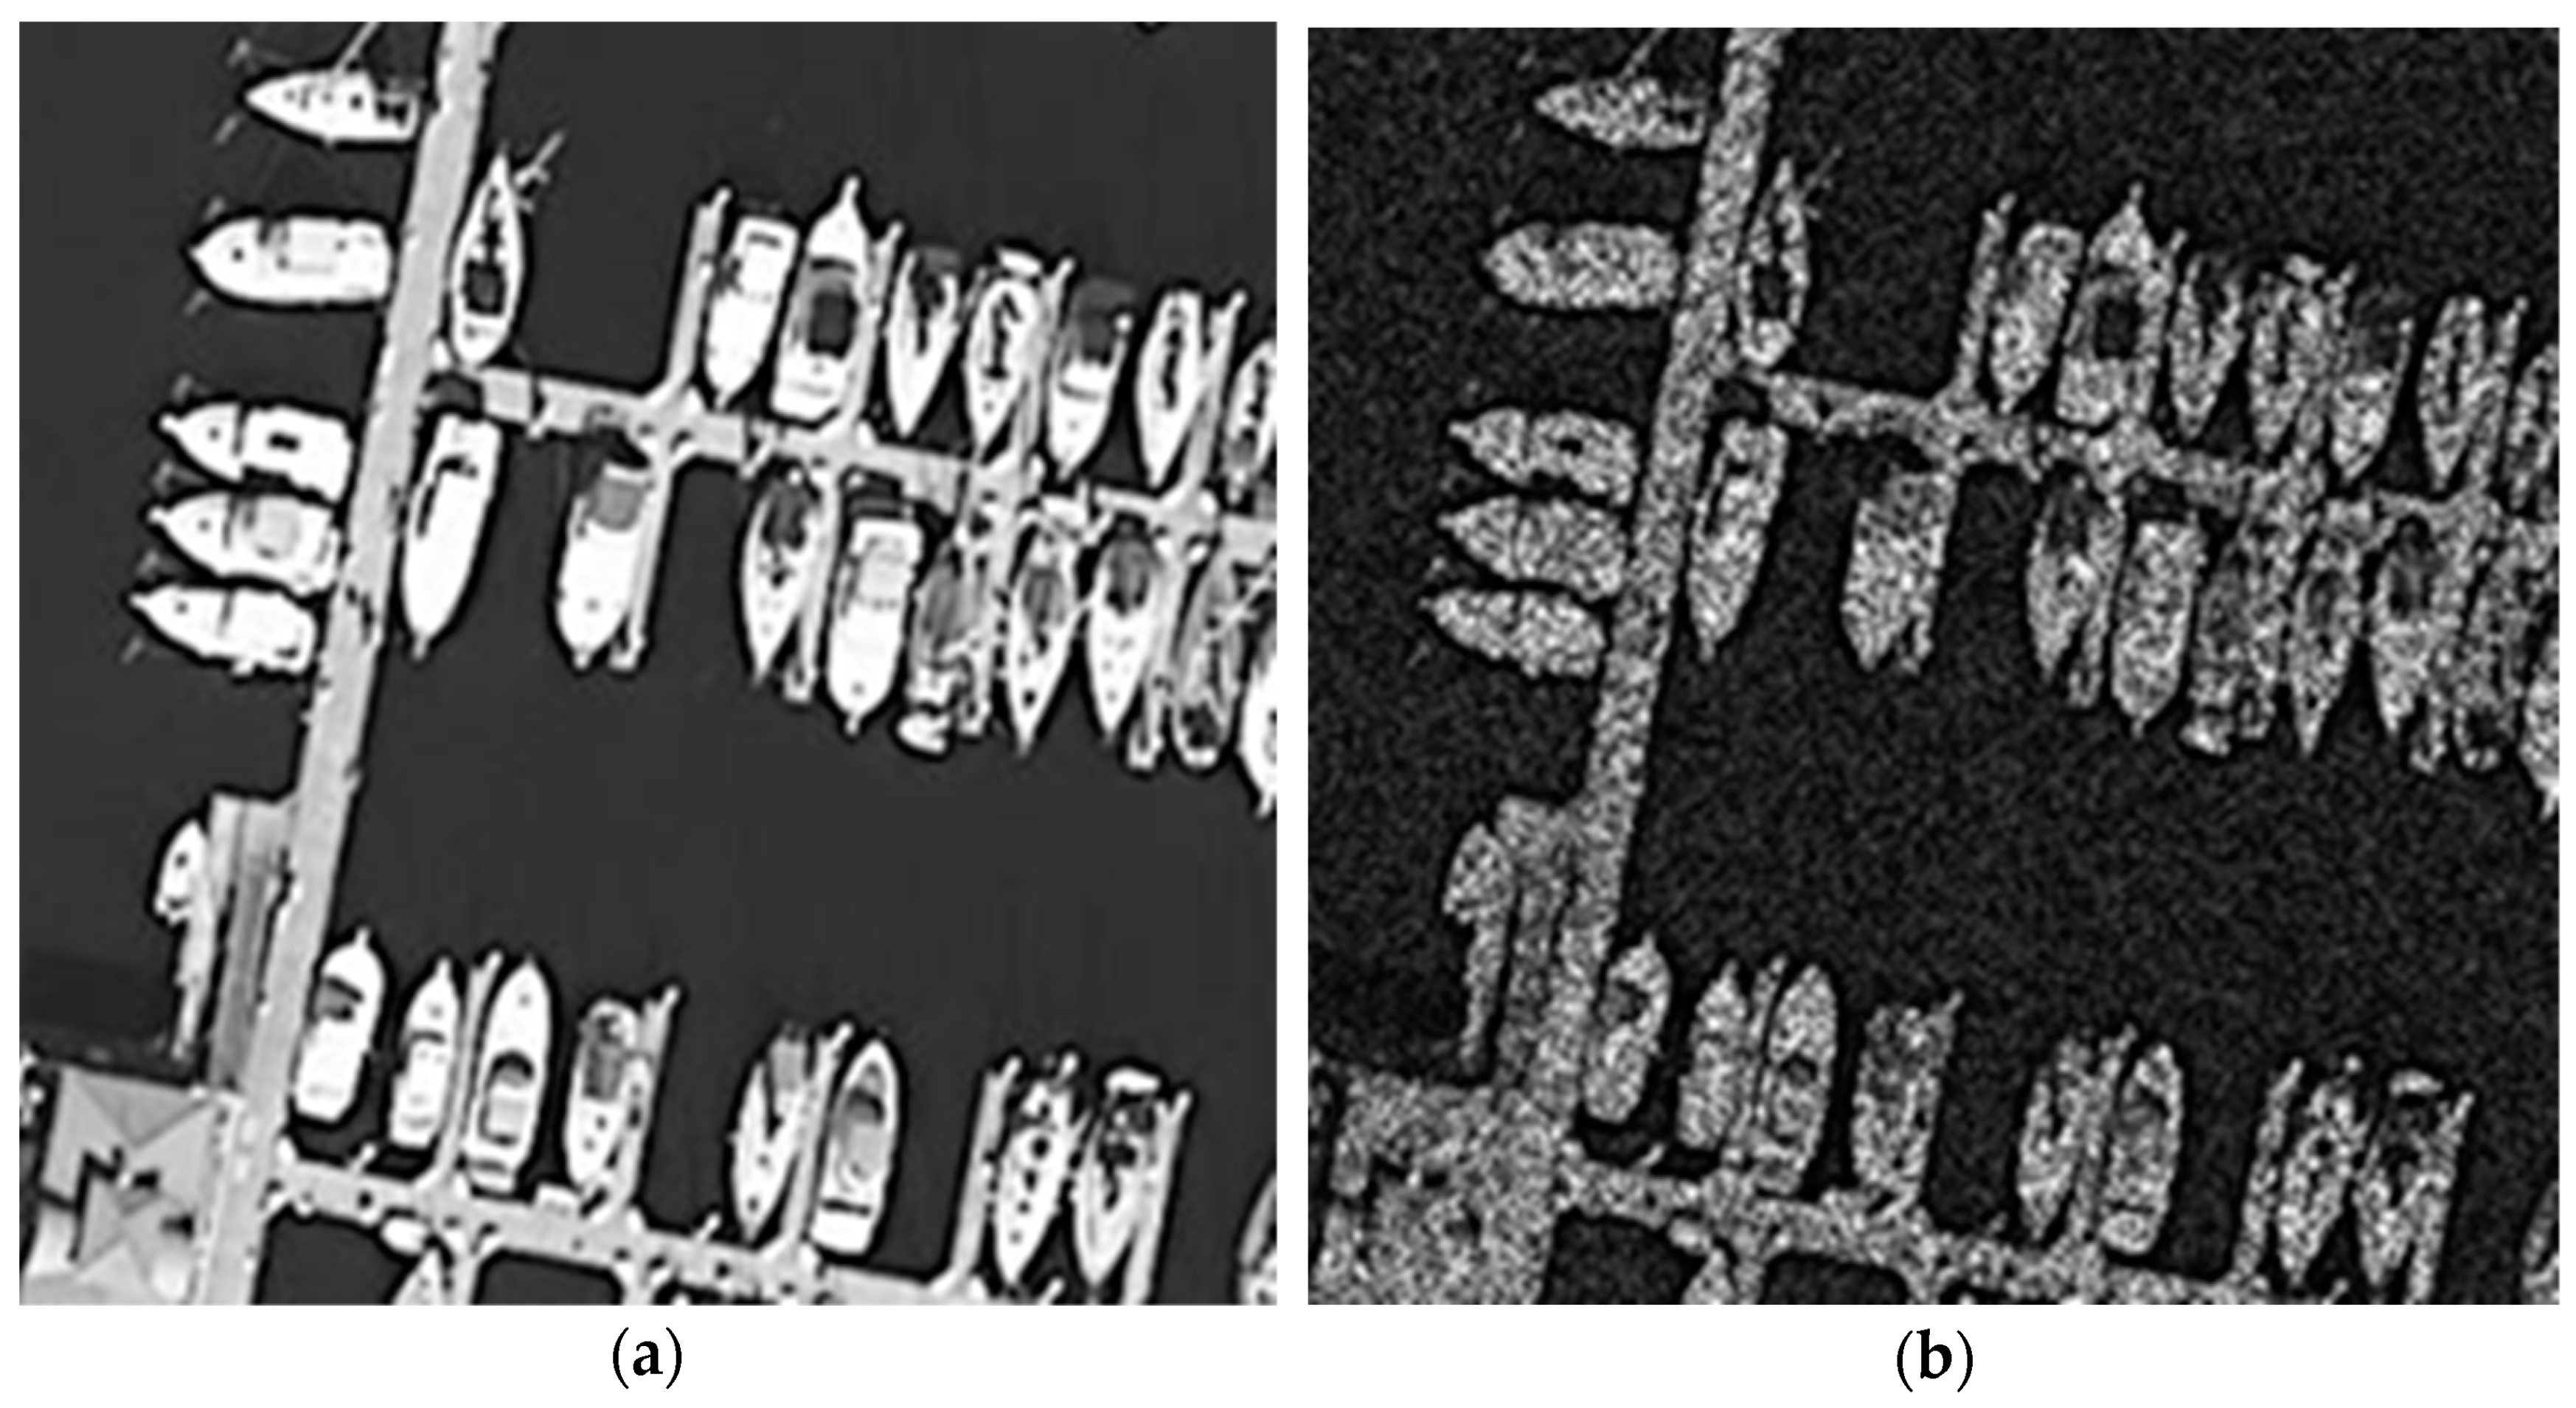
\includegraphics[width=0.75\textwidth]{../research-resources/SAR/sar-speckle.png}
	\caption{a. Optical Image; b. SAR Image with speckle noise}
\end{figure}

\indent Given the availability of remote sensed data and their different observed properties, there is much to be learned about the state of the sea ice by corroborating these data sources with each other. Uniquely, the corroboration of a SAR image with precise LiDAR measurements suggests the possibility of developing a convolutional neural network (CNN) to accurately predict sea ice thickness using expansive SAR imaging. Doing so successfully would effectively map IS-2's precision onto the weather agnostic, extensive imaging gathered by SAR satellites, thus allowing for local scale analysis of sea ice across large regions.


 \indent Given that ice thickness is not a property directly measured by LiDAR nor captured in SAR imagery, sets of assumptions need to be made to deduce the property through related measurements. A leading paradigm in modeling ice thickness is through the assumption of hydrostatic equilibrium \cite{ICESat-2-L4-Product, Hutchings_Heil_Lecomte_Stevens_Steer_Lieser_2015, Forsström_Gerland_Pedersen_2011}, in which the properties of the ice sheet are deduced based upon the fact that the ice is buoyant in sea water (Figure 1.3). In this assumption, LiDAR measurements retrieve the elevations of the snow covered ice-surface in relation to the sea surface, and statistically infer the sea ice surface height. It's possible to relate the ice's total thickness to these elevation measurements by combining these relative heights with their associated substance densities (Equation 1.1). NASA's IS-2 L4 Along-Track Sea Ice Thickness product is a closely related example of this topic, and produced arctic ice thickness results between October 2018 and May 2022 \cite{ICESat-2-L4-Product}.
 \begin{figure}[]
	\centering
	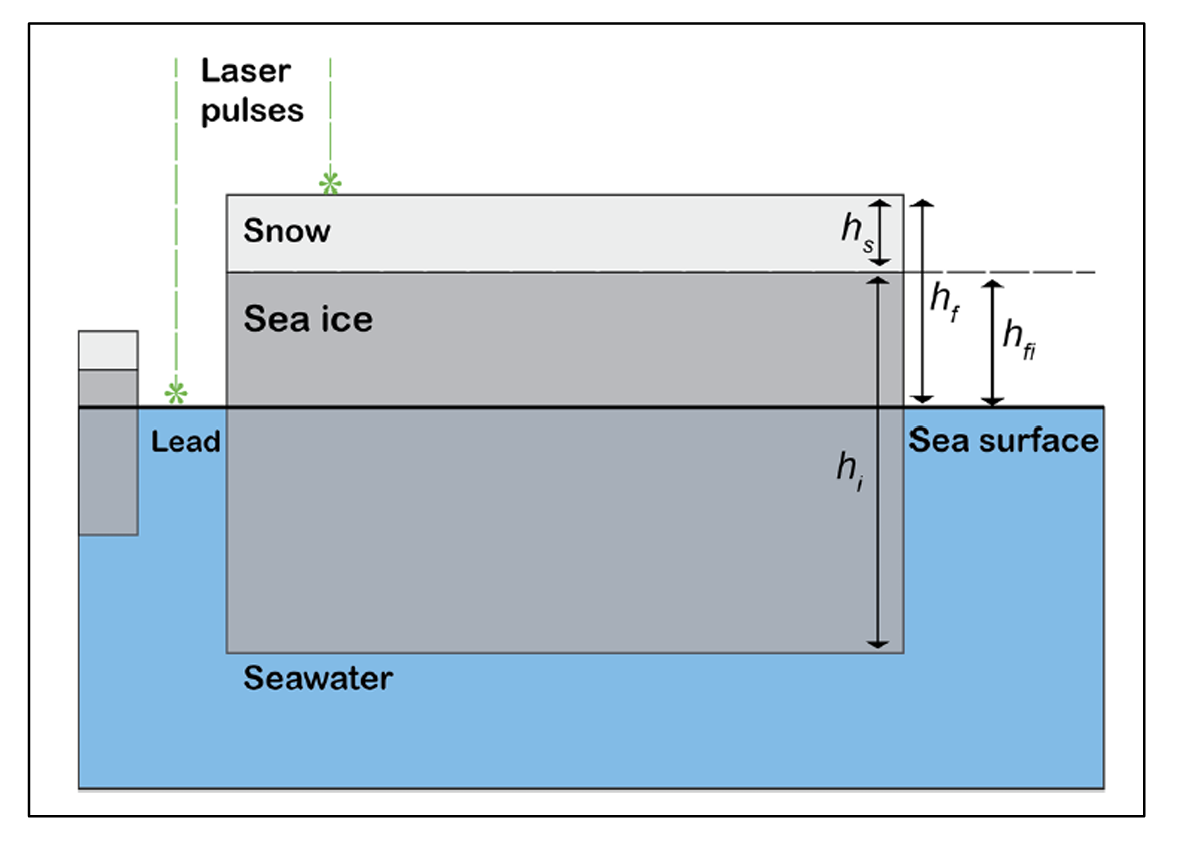
\includegraphics[width=.8\textwidth]{../research-resources/ice-sat-2/hydro-static-equillibrium.png}
	\caption{Ice Thickness Isostatic Assumption} \cite{ICESat-2-L4-Product}
	\label{fig:hydro-static-diagram}
\end{figure}

There are critiques with the established hydrostatic model. Ice density at a local scale is a variable property - it's dependent on factors like salinity, temperature, air volume and exposure \cite{sea-ice-properties}, and has a large enough observable difference that ice can be reliably classified into first and multi-year ice by SAR imaging alone \cite{SAR-U-Net}. Some studies delineate ice density by whether it's above or below the waterline, but find that air-rich above water ice only contributes to 10\% of the total density of the ice sheet. Given the variability, the exact local density of sea ice in the remote arctic is ephemeral, but generally agreed upon to be between 900-940 $\frac{kg}{m^3}$, with some studies proposing a slightly wider range of 892-945 \cite{sea-ice-properties}. As a concrete example though, IS-2's L4 product settled to use a value of 916 $\frac{kg}{m^3}$ for ice above and below the waterline.

\begin{equation}
	\label{eq:isostatic-equilibrium}
	\displaystyle h_i=\frac{\displaystyle h_f\rho_w}{(\rho_w-\rho_i)}+\frac{\displaystyle h_s(\rho_s-\rho_w)}{(\rho_w-\rho_i)}
\end{equation}
where:
\begin{align*}
 \displaystyle h_i    &=  \text{Sea ice thickness (m)} &  \rho_i 							&=  \text{Density of sea ice }(900-940 \frac{kg}{m^3}) \\   %	It'd be perfect to place the diagram of the sheet in the white space generated here in latex
 \rho_w 							&=  \text{Density of water} 		 & 	\rho_s							&=  \text{Density of snow} \\   %	It'd be perfect to place the diagram of the sheet in the white space generated here in latex
 \displaystyle h_f    &=  \text{Freeboard height (m)}  & 	\displaystyle h_s   &=  \text{Snow depth (m)} \\   %	It'd be perfect to place the diagram of the sheet in the white space generated here in latex
\end{align*}

Even with the established hydrostatic model in place to infer sea ice thickness from remote sensing methods, there is an innate problem with the corroboration of SAR and LiDAR. IS-2 has an orbit cycle of 91 days, meaning each location is surveyed only once nearly every 3 months \cite{ICESat-2-ATL10-Product}, while SN-2 orbits nearly once every 5 days \cite{copernicusSentinel2Missions}. It may appear that there should be plenty of data available given the semi-frequent opportunity for coincidence, but given SN-2's best resolution of 10m, any correlation with IS-2's 17m footprint leads to single pixels of information.


The remainder of the thesis will be split between discussing the data collection and machine learning model experimentation. The data collection section will discuss the procedure for obtaining datasets of interest, as well as some intermediate efforts done to promote accuracy. The  experimentation will use the collected data to develop a convolutional neural network to explore the feasibility of using such a source of data for deep learning models.